\subsubsection{Swarm AEJ data products}

\begin{verbatim}
import datetime
import matplotlib.pyplot as plt
import numpy as np
import pathlib

import geospacelab.visualization.mpl.dashboards as dashboards
\end{verbatim}

\paragraph{Swarm AEJ LPS data product}

\subparagraph{Overview with a long time span}

\begin{verbatim}
def test_swarm_AEJ_LPL_overview():
    """Test Swarm AEJ/LPL data product
    
    """
    dt_fr = datetime.datetime(2024, 5, 10, 12, 0)
    dt_to = datetime.datetime(2024, 5, 11, 12, 0)

    db = dashboards.TSDashboard(
        dt_fr=dt_fr, dt_to=dt_to, figure_config={'figsize': (8, 8)},
        )

    ds = db.dock(
        datasource_contents=['esa_eo', 'swarm', 'l2daily', 'aej_lpl'], 
        product_version='latest', # 'latest' (default), '0301', 
        sat_id='C', add_APEX=True, add_AACGM=True)

    glat = ds['GEO_LAT']
    glon = ds['GEO_LON']
    J_N = ds['J_N']
    J_E = ds['J_E']
    J_QD = ds['J_QD']
    
    panel_layouts = [
        [J_N, J_E],
        [J_QD],
        [glat, [glon]]
    ]

    db.set_layout(panel_layouts=panel_layouts)
    db.draw()
    db.add_title(title='Swarm -{} AEJ/LPL Overview'.format(ds.sat_id), fontsize='medium', append_time=True)

    db.show()
    
test_swarm_AEJ_LPL_overview()
\end{verbatim}

\begin{verbatim}
Create a new figure: Figure(800x800).
\end{verbatim}

\begin{verbatim}
Load IGRF coefficients ...
\end{verbatim}

\begin{verbatim}
Searching the data product "AEJ_LPL" with the version "latest" on the server...
INFO: Indexing the files for the product AEJ_LPL of the satellite C ...
The file [PosixPath('/data/afys -ionosphere/data/ESA/SWARM/Level2daily/AEJ_LPL/0301/Sat_C/2024/SW_OPER_AEJCLPL_2F_20240510T000000_20240510T235959_0301.cdf')] already exists: skip downloading.
The file [PosixPath('/data/afys -ionosphere/data/ESA/SWARM/Level2daily/AEJ_LPL/0301/Sat_C/2024/SW_OPER_AEJCLPL_2F_20240511T000000_20240511T235959_0301.cdf')] already exists: skip downloading.
resetting environment variable IGRF_COEFFS in python script
resetting environment variable AACGM_v2_DAT_PREFIX in python script
non -default coefficient files may be specified by running aacgmv2.wrapper.set_coeff_path before any other functions
/opt/anaconda3/envs/Swarm/lib/python3.12/site -packages/numpy/_core/numeric.py:476: RuntimeWarning: invalid value encountered in cast
  multiarray.copyto(res, fill_value, casting='unsafe')
\end{verbatim}

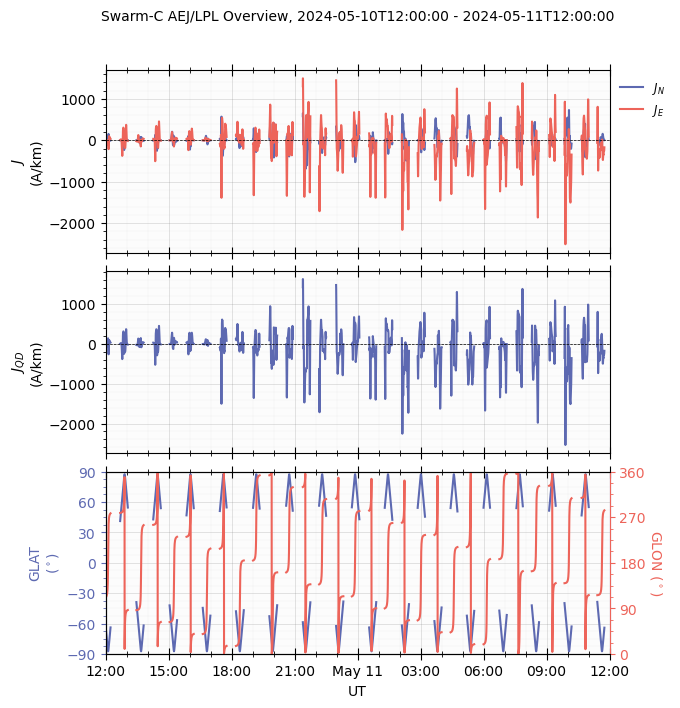
\includegraphics[width=0.7\linewidth]{files/395de7af547d1f43c3c00947d4da195a.png}

\subparagraph{Zoomed-in view with a short time span}

\begin{verbatim}
def test_swarm_AEJ_LPL_zoom():
    """Test Swarm AEJ/LPL data product
    
    """
    dt_fr = datetime.datetime(2024, 5, 10, 20, 30)
    dt_to = datetime.datetime(2024, 5, 10, 21, 0)

    db = dashboards.TSDashboard(
        dt_fr=dt_fr, dt_to=dt_to, figure_config={'figsize': (8, 8)},
        timeline_extra_labels=['GEO_LAT', 'GEO_LON', 'APEX_LAT', 'APEX_LON', 'APEX_MLT',] 
        )

    ds = db.dock(datasource_contents=['esa_eo', 'swarm', 'l2daily', 'aej_lpl'], sat_id='C', add_APEX=True, add_AACGM=True)

    glat = ds['GEO_LAT']
    glon = ds['GEO_LON']
    J_N = ds['J_N']
    J_E = ds['J_E']
    J_QD = ds['J_QD']
    
    panel_layouts = [
        [J_N, J_E],
        [J_QD],
        [glat, [glon]]
    ]

    db.set_layout(panel_layouts=panel_layouts)
    db.draw()
    db.add_title(title='Swarm -{} AEJ/LPL Zoom'.format(ds.sat_id), fontsize='medium', append_time=True)
    
    db.show()
test_swarm_AEJ_LPL_zoom()
\end{verbatim}

\begin{verbatim}
Create a new figure: Figure(800x800).
Searching the data product "AEJ_LPL" with the version "latest" on the server...
The file [PosixPath('/data/afys -ionosphere/data/ESA/SWARM/Level2daily/AEJ_LPL/0301/Sat_C/2024/SW_OPER_AEJCLPL_2F_20240510T000000_20240510T235959_0301.cdf')] already exists: skip downloading.
\end{verbatim}

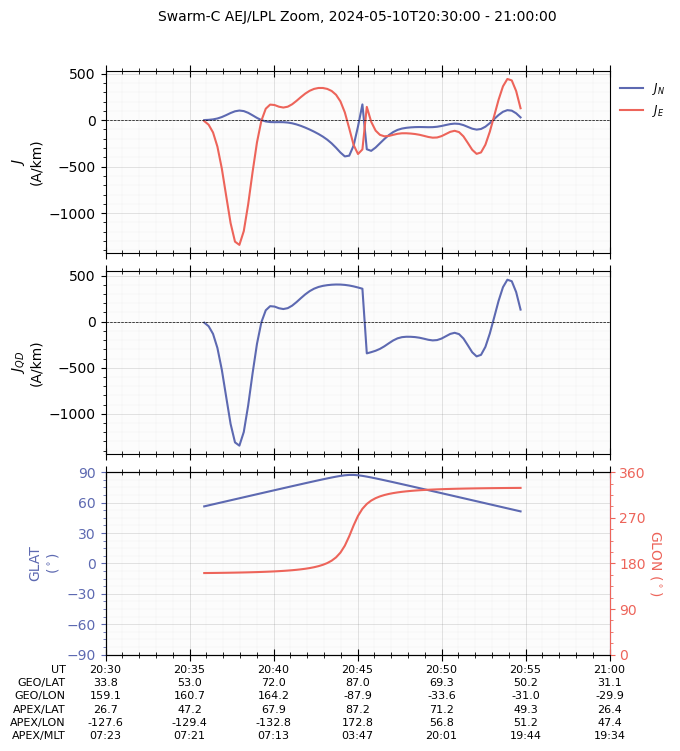
\includegraphics[width=0.7\linewidth]{files/a3e38009b0b655142392719442c30737.png}

\paragraph{Swarm AEJ LPS data product}

\subparagraph{Overview with a long time span}

\begin{verbatim}
def test_swarm_AEJ_LPS_overview():
    """Test Swarm AEJ/LPS data product
    
    """
    dt_fr = datetime.datetime(2024, 5, 10, 12, 0)
    dt_to = datetime.datetime(2024, 5, 11, 12, 0)

    db = dashboards.TSDashboard(
        dt_fr=dt_fr, dt_to=dt_to, figure_config={'figsize': (8, 8)},
        )

    ds = db.dock(datasource_contents=['esa_eo', 'swarm', 'l2daily', 'aej_lps'], sat_id='C', add_APEX=True, add_AACGM=True)

    glat = ds['GEO_LAT']
    glon = ds['GEO_LON']
    J_CF_N = ds['J_CF_N']
    J_CF_E = ds['J_CF_E']
    J_DF_N = ds['J_DF_N']
    J_DF_E = ds['J_DF_E']
    J_r = ds['J_r']
    
    panel_layouts = [
        [J_CF_N, J_CF_E],
        [J_DF_N, J_DF_E],
        [J_r],
        [glat, [glon]]
    ]

    db.set_layout(panel_layouts=panel_layouts)
    db.draw()
    db.add_title(title='Swarm -{} AEJ/LPS Overview'.format(ds.sat_id), fontsize='medium', append_time=True)

    db.show()
test_swarm_AEJ_LPS_overview()
\end{verbatim}

\begin{verbatim}
Create a new figure: Figure(800x800).
Searching the data product "AEJ_LPS" with the version "latest" on the server...
INFO: Indexing the files for the product AEJ_LPS of the satellite C ...
The file [PosixPath('/data/afys -ionosphere/data/ESA/SWARM/Level2daily/AEJ_LPS/0101/Sat_C/2024/SW_OPER_AEJCLPS_2F_20240510T000000_20240510T235959_0101.cdf')] already exists: skip downloading.
The file [PosixPath('/data/afys -ionosphere/data/ESA/SWARM/Level2daily/AEJ_LPS/0101/Sat_C/2024/SW_OPER_AEJCLPS_2F_20240511T000000_20240511T235959_0101.cdf')] already exists: skip downloading.
\end{verbatim}

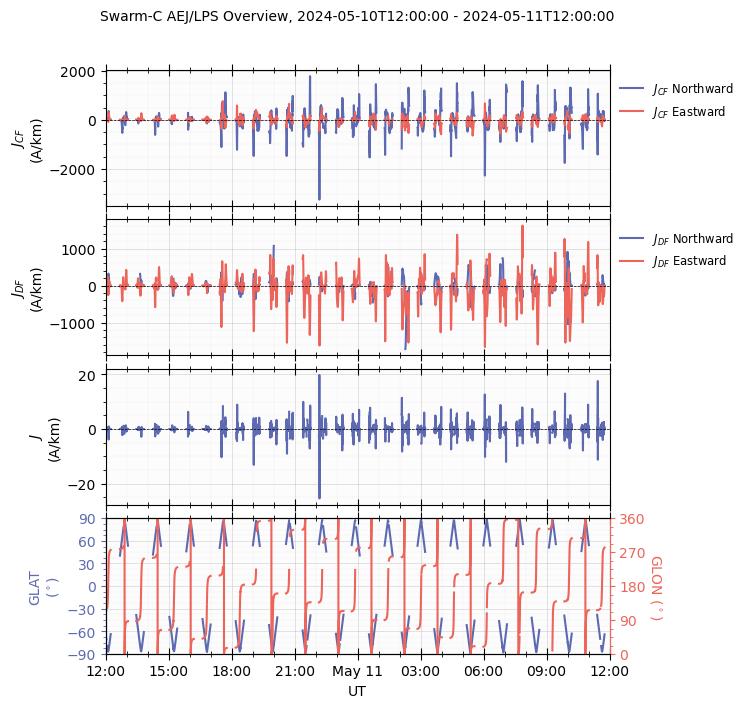
\includegraphics[width=0.7\linewidth]{files/82eb2efe96a89c248afb93adecff475f.png}

\subparagraph{Zoomed-in view with a short time span}

\begin{verbatim}
def test_swarm_AEJ_LPS_zoom():
    """Test Swarm AEJ/LPS data product
    
    """
    dt_fr = datetime.datetime(2024, 5, 10, 20, 30)
    dt_to = datetime.datetime(2024, 5, 10, 21, 0)

    db = dashboards.TSDashboard(
        dt_fr=dt_fr, dt_to=dt_to, figure_config={'figsize': (8, 8)},
        timeline_extra_labels=['GEO_LAT', 'GEO_LON', 'APEX_LAT', 'APEX_LON', 'APEX_MLT',] 
        )

    ds = db.dock(datasource_contents=['esa_eo', 'swarm', 'l2daily', 'aej_lps'], sat_id='C', add_APEX=True, add_AACGM=True)

    glat = ds['GEO_LAT']
    glon = ds['GEO_LON']
    J_CF_N = ds['J_CF_N']
    J_CF_E = ds['J_CF_E']
    J_DF_N = ds['J_DF_N']
    J_DF_E = ds['J_DF_E']
    J_r = ds['J_r']
    
    panel_layouts = [
        [J_CF_N, J_CF_E],
        [J_DF_N, J_DF_E],
        [J_r],
        [glat, [glon]]
    ]

    db.set_layout(panel_layouts=panel_layouts)
    db.draw()
    db.add_title(title='Swarm -{} AEJ/LPS Zoom'.format(ds.sat_id), fontsize='medium', append_time=True)
    db.show()
test_swarm_AEJ_LPS_zoom()
\end{verbatim}

\begin{verbatim}
Create a new figure: Figure(800x800).
Searching the data product "AEJ_LPS" with the version "latest" on the server...
The file [PosixPath('/data/afys -ionosphere/data/ESA/SWARM/Level2daily/AEJ_LPS/0101/Sat_C/2024/SW_OPER_AEJCLPS_2F_20240510T000000_20240510T235959_0101.cdf')] already exists: skip downloading.
\end{verbatim}

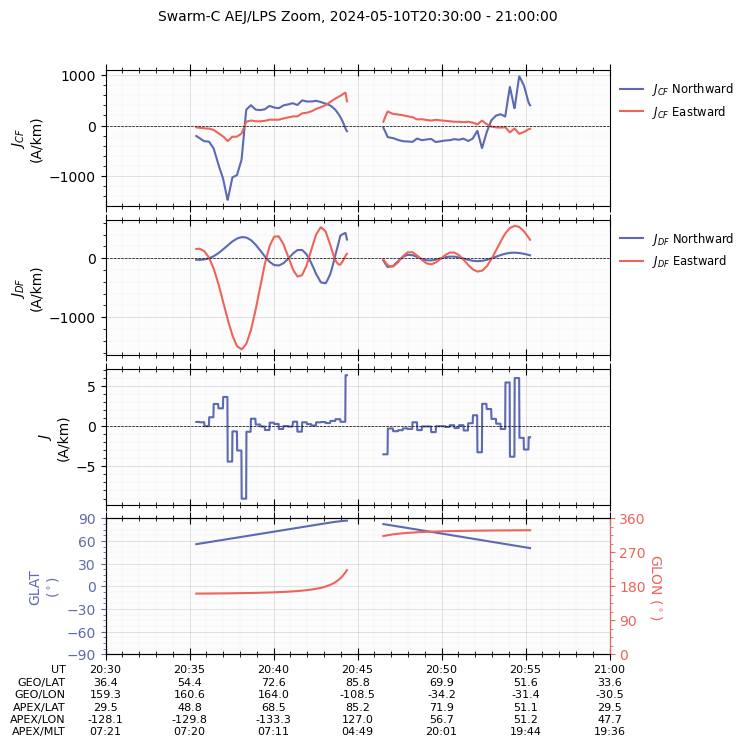
\includegraphics[width=0.7\linewidth]{files/317268c2a6e1aea8a2b62e50bc7510d4.png}

\paragraph{Swarm AEJ PBL data product}

\subparagraph{Overview with a long time span}

\begin{verbatim}
def test_swarm_AEJ_PBL_overview():
    """Test Swarm AEJ/PBL data product
    
    """
    dt_fr = datetime.datetime(2024, 5, 10, 12, 0)
    dt_to = datetime.datetime(2024, 5, 11, 12, 0)

    db = dashboards.TSDashboard(
        dt_fr=dt_fr, dt_to=dt_to, figure_config={'figsize': (8, 8)},
        )

    ds = db.dock(datasource_contents=['esa_eo', 'swarm', 'l2daily', 'aej_pbl'], sat_id='C', add_APEX=True, add_AACGM=True)

    panel_layouts = [
        [ds['WEJ_PEAK'], ds['EEJ_PEAK']],
        [
            ds['GEO_LAT_WEJ_PB'],
            ds['GEO_LAT_WEJ_PEAK'], 
            ds['GEO_LAT_WEJ_EB'],
            ds['GEO_LAT_EEJ_PB'],
            ds['GEO_LAT_EEJ_PEAK'],
            ds['GEO_LAT_EEJ_EB'],
        ],
        [
            ds['QD_LAT_WEJ_PB'],
            ds['QD_LAT_WEJ_PEAK'],
            ds['QD_LAT_WEJ_EB'],
            ds['QD_LAT_EEJ_PB'],
            ds['QD_LAT_EEJ_PEAK'],
            ds['QD_LAT_EEJ_EB'],
        ],
        [
            ds['QUALITY_FLAG_BIN_AUX'],
        ],
    ]

    db.set_layout(panel_layouts=panel_layouts)
    db.draw()
    db.add_title(title='Swarm -{} AEJ/PBL Overview'.format(ds.sat_id), fontsize='medium', append_time=True)

    db.show()
test_swarm_AEJ_PBL_overview()
\end{verbatim}

\begin{verbatim}
Create a new figure: Figure(800x800).
Searching the data product "AEJ_PBL" with the version "latest" on the server...
INFO: Indexing the files for the product AEJ_PBL of the satellite C ...
The file [PosixPath('/data/afys -ionosphere/data/ESA/SWARM/Level2daily/AEJ_PBL/0301/Sat_C/2024/SW_OPER_AEJCPBL_2F_20240101T000000_20241231T235959_0301.cdf')] already exists: skip downloading.
/opt/anaconda3/envs/Swarm/lib/python3.12/site -packages/apexpy/apex.py:556: RuntimeWarning: invalid value encountered in <lambda> (vectorized)
  alat, alon = self._geo2apex(glat, glon, height)
/opt/anaconda3/envs/Swarm/lib/python3.12/site -packages/apexpy/apex.py:559: UserWarning: Apex latitude set to NaN where undefined (apex height may be < reference height)
  warnings.warn(''.join(['Apex latitude set to NaN where undefined ',
/opt/anaconda3/envs/Swarm/lib/python3.12/site -packages/apexpy/apex.py:559: UserWarning: Apex latitude set to NaN where undefined (apex height may be < reference height)
  warnings.warn(''.join(['Apex latitude set to NaN where undefined ',
/opt/anaconda3/envs/Swarm/lib/python3.12/site -packages/apexpy/apex.py:559: UserWarning: Apex latitude set to NaN where undefined (apex height may be < reference height)
  warnings.warn(''.join(['Apex latitude set to NaN where undefined ',
/opt/anaconda3/envs/Swarm/lib/python3.12/site -packages/apexpy/apex.py:559: UserWarning: Apex latitude set to NaN where undefined (apex height may be < reference height)
  warnings.warn(''.join(['Apex latitude set to NaN where undefined ',
/opt/anaconda3/envs/Swarm/lib/python3.12/site -packages/apexpy/apex.py:559: UserWarning: Apex latitude set to NaN where undefined (apex height may be < reference height)
  warnings.warn(''.join(['Apex latitude set to NaN where undefined ',
/opt/anaconda3/envs/Swarm/lib/python3.12/site -packages/apexpy/apex.py:559: UserWarning: Apex latitude set to NaN where undefined (apex height may be < reference height)
  warnings.warn(''.join(['Apex latitude set to NaN where undefined ',
/opt/anaconda3/envs/Swarm/lib/python3.12/site -packages/apexpy/apex.py:559: UserWarning: Apex latitude set to NaN where undefined (apex height may be < reference height)
  warnings.warn(''.join(['Apex latitude set to NaN where undefined ',
/opt/anaconda3/envs/Swarm/lib/python3.12/site -packages/apexpy/apex.py:559: UserWarning: Apex latitude set to NaN where undefined (apex height may be < reference height)
  warnings.warn(''.join(['Apex latitude set to NaN where undefined ',
/opt/anaconda3/envs/Swarm/lib/python3.12/site -packages/apexpy/apex.py:559: UserWarning: Apex latitude set to NaN where undefined (apex height may be < reference height)
  warnings.warn(''.join(['Apex latitude set to NaN where undefined ',
/opt/anaconda3/envs/Swarm/lib/python3.12/site -packages/apexpy/apex.py:559: UserWarning: Apex latitude set to NaN where undefined (apex height may be < reference height)
  warnings.warn(''.join(['Apex latitude set to NaN where undefined ',
/opt/anaconda3/envs/Swarm/lib/python3.12/site -packages/apexpy/apex.py:559: UserWarning: Apex latitude set to NaN where undefined (apex height may be < reference height)
  warnings.warn(''.join(['Apex latitude set to NaN where undefined ',
/opt/anaconda3/envs/Swarm/lib/python3.12/site -packages/apexpy/apex.py:559: UserWarning: Apex latitude set to NaN where undefined (apex height may be < reference height)
  warnings.warn(''.join(['Apex latitude set to NaN where undefined ',
\end{verbatim}

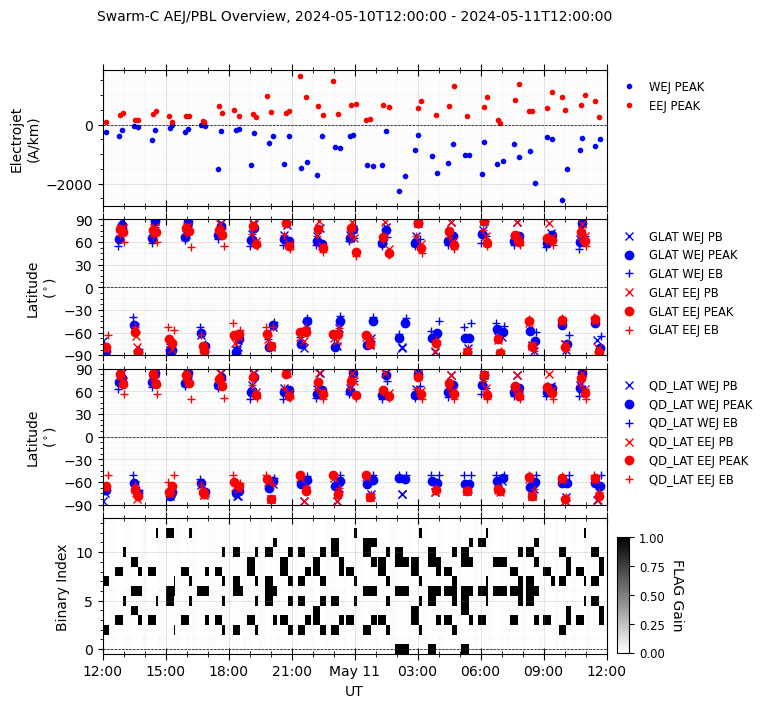
\includegraphics[width=0.7\linewidth]{files/72f8bfc9edf3f1fcc246fd249b049a13.png}

\subparagraph{Zoomed-in view with a short time span}

\begin{verbatim}
def test_swarm_AEJ_PBL_zoom():
    """Test Swarm AEJ/PBL data product
    
    """
    dt_fr = datetime.datetime(2024, 5, 10, 20, 30)
    dt_to = datetime.datetime(2024, 5, 10, 21, 0)

    db = dashboards.TSDashboard(
        dt_fr=dt_fr, dt_to=dt_to, figure_config={'figsize': (8, 8)},
        # timeline_extra_labels=['GEO_LAT', 'GEO_LON', 'APEX_LAT', 'APEX_LON', 'APEX_MLT',]  # Not applicable for very scattered data points like AEJ_PBL peaks
        )

    ds = db.dock(datasource_contents=['esa_eo', 'swarm', 'l2daily', 'aej_pbl'], sat_id='C', add_APEX=True, add_AACGM=True)

    panel_layouts = [
        [ds['WEJ_PEAK'], ds['EEJ_PEAK']],
        [
            ds['GEO_LAT_WEJ_PB'],
            ds['GEO_LAT_WEJ_PEAK'], 
            ds['GEO_LAT_WEJ_EB'],
            ds['GEO_LAT_EEJ_PB'],
            ds['GEO_LAT_EEJ_PEAK'],
            ds['GEO_LAT_EEJ_EB'],
            ],
        [
            ds['QD_LAT_WEJ_PB'],
            ds['QD_LAT_WEJ_PEAK'],
            ds['QD_LAT_WEJ_EB'],
            ds['QD_LAT_EEJ_PB'],
            ds['QD_LAT_EEJ_PEAK'],
            ds['QD_LAT_EEJ_EB'],
            ],
        [
            ds['QUALITY_FLAG_BIN_AUX'],
        ],
    ]

    db.set_layout(panel_layouts=panel_layouts)
    db.draw()
    db.add_title(title='Swarm -{} AEJ/PBL Zoom'.format(ds.sat_id), fontsize='medium', append_time=True)
    
    db.show()
test_swarm_AEJ_PBL_zoom()
\end{verbatim}

\begin{verbatim}
Create a new figure: Figure(800x800).
Searching the data product "AEJ_PBL" with the version "latest" on the server...
The file [PosixPath('/data/afys -ionosphere/data/ESA/SWARM/Level2daily/AEJ_PBL/0301/Sat_C/2024/SW_OPER_AEJCPBL_2F_20240101T000000_20241231T235959_0301.cdf')] already exists: skip downloading.
\end{verbatim}

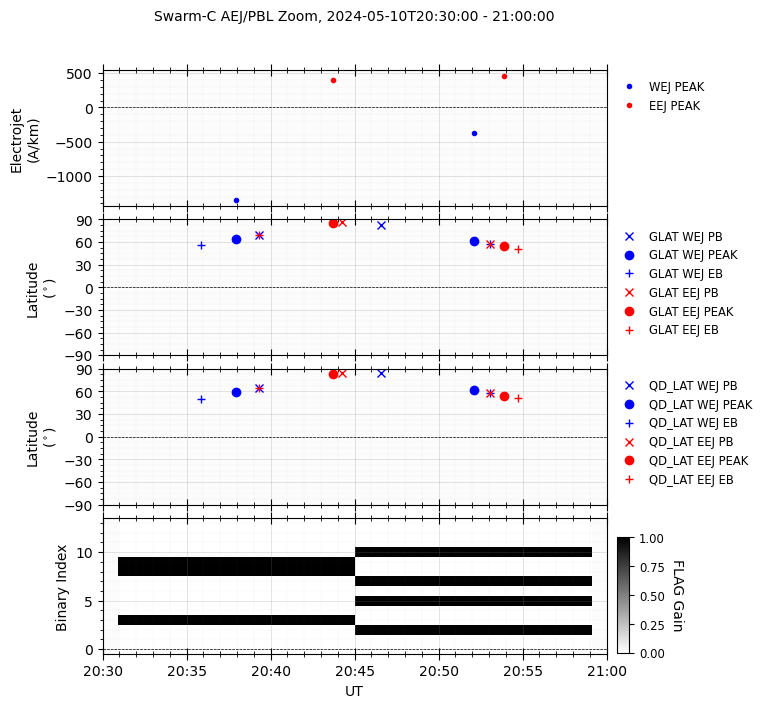
\includegraphics[width=0.7\linewidth]{files/eaf3f337786bc162074587a70df71bec.png}

\paragraph{Swarm AEJ PBS data product}

\subparagraph{Overview with a long time span}

\begin{verbatim}
def test_swarm_AEJ_PBS_overview():
    """Test Swarm AEJ/PBS data product
    
    """
    dt_fr = datetime.datetime(2024, 5, 10, 12, 0)
    dt_to = datetime.datetime(2024, 5, 11, 12, 0)

    db = dashboards.TSDashboard(
        dt_fr=dt_fr, dt_to=dt_to, figure_config={'figsize': (8, 8)},
        )

    ds = db.dock(datasource_contents=['esa_eo', 'swarm', 'l2daily', 'aej_pbs'], sat_id='C', add_APEX=True, add_AACGM=True)

    panel_layouts = [
        [ds['WEJ_PEAK'], ds['EEJ_PEAK']],
        [
            ds['GEO_LAT_WEJ_PB'],
            ds['GEO_LAT_WEJ_PEAK'], 
            ds['GEO_LAT_WEJ_EB'],
            ds['GEO_LAT_EEJ_PB'],
            ds['GEO_LAT_EEJ_PEAK'],
            ds['GEO_LAT_EEJ_EB'],
        ],
        [
            ds['QD_LAT_WEJ_PB'],
            ds['QD_LAT_WEJ_PEAK'],
            ds['QD_LAT_WEJ_EB'],
            ds['QD_LAT_EEJ_PB'],
            ds['QD_LAT_EEJ_PEAK'],
            ds['QD_LAT_EEJ_EB'],
        ],
        [
            ds['QUALITY_FLAG_BIN_AUX'],
        ],
    ]

    db.set_layout(panel_layouts=panel_layouts)
    db.draw()
    db.add_title(title='Swarm -{} AEJ/PBS Overview'.format(ds.sat_id), fontsize='medium', append_time=True)

    db.show()
test_swarm_AEJ_PBS_overview()
\end{verbatim}

\begin{verbatim}
Create a new figure: Figure(800x800).
Searching the data product "AEJ_PBS" with the version "latest" on the server...
INFO: Indexing the files for the product AEJ_PBS of the satellite C ...
The file [PosixPath('/data/afys -ionosphere/data/ESA/SWARM/Level2daily/AEJ_PBS/0101/Sat_C/2024/SW_OPER_AEJCPBS_2F_20240101T000000_20241031T235959_0101.cdf')] already exists: skip downloading.
/opt/anaconda3/envs/Swarm/lib/python3.12/site -packages/apexpy/apex.py:559: UserWarning: Apex latitude set to NaN where undefined (apex height may be < reference height)
  warnings.warn(''.join(['Apex latitude set to NaN where undefined ',
/opt/anaconda3/envs/Swarm/lib/python3.12/site -packages/apexpy/apex.py:559: UserWarning: Apex latitude set to NaN where undefined (apex height may be < reference height)
  warnings.warn(''.join(['Apex latitude set to NaN where undefined ',
/opt/anaconda3/envs/Swarm/lib/python3.12/site -packages/apexpy/apex.py:559: UserWarning: Apex latitude set to NaN where undefined (apex height may be < reference height)
  warnings.warn(''.join(['Apex latitude set to NaN where undefined ',
/opt/anaconda3/envs/Swarm/lib/python3.12/site -packages/apexpy/apex.py:559: UserWarning: Apex latitude set to NaN where undefined (apex height may be < reference height)
  warnings.warn(''.join(['Apex latitude set to NaN where undefined ',
/opt/anaconda3/envs/Swarm/lib/python3.12/site -packages/apexpy/apex.py:559: UserWarning: Apex latitude set to NaN where undefined (apex height may be < reference height)
  warnings.warn(''.join(['Apex latitude set to NaN where undefined ',
/opt/anaconda3/envs/Swarm/lib/python3.12/site -packages/apexpy/apex.py:559: UserWarning: Apex latitude set to NaN where undefined (apex height may be < reference height)
  warnings.warn(''.join(['Apex latitude set to NaN where undefined ',
/opt/anaconda3/envs/Swarm/lib/python3.12/site -packages/apexpy/apex.py:559: UserWarning: Apex latitude set to NaN where undefined (apex height may be < reference height)
  warnings.warn(''.join(['Apex latitude set to NaN where undefined ',
/opt/anaconda3/envs/Swarm/lib/python3.12/site -packages/apexpy/apex.py:559: UserWarning: Apex latitude set to NaN where undefined (apex height may be < reference height)
  warnings.warn(''.join(['Apex latitude set to NaN where undefined ',
/opt/anaconda3/envs/Swarm/lib/python3.12/site -packages/apexpy/apex.py:559: UserWarning: Apex latitude set to NaN where undefined (apex height may be < reference height)
  warnings.warn(''.join(['Apex latitude set to NaN where undefined ',
/opt/anaconda3/envs/Swarm/lib/python3.12/site -packages/apexpy/apex.py:559: UserWarning: Apex latitude set to NaN where undefined (apex height may be < reference height)
  warnings.warn(''.join(['Apex latitude set to NaN where undefined ',
/opt/anaconda3/envs/Swarm/lib/python3.12/site -packages/apexpy/apex.py:559: UserWarning: Apex latitude set to NaN where undefined (apex height may be < reference height)
  warnings.warn(''.join(['Apex latitude set to NaN where undefined ',
/opt/anaconda3/envs/Swarm/lib/python3.12/site -packages/apexpy/apex.py:559: UserWarning: Apex latitude set to NaN where undefined (apex height may be < reference height)
  warnings.warn(''.join(['Apex latitude set to NaN where undefined ',
/opt/anaconda3/envs/Swarm/lib/python3.12/site -packages/apexpy/apex.py:559: UserWarning: Apex latitude set to NaN where undefined (apex height may be < reference height)
  warnings.warn(''.join(['Apex latitude set to NaN where undefined ',
/opt/anaconda3/envs/Swarm/lib/python3.12/site -packages/apexpy/apex.py:559: UserWarning: Apex latitude set to NaN where undefined (apex height may be < reference height)
  warnings.warn(''.join(['Apex latitude set to NaN where undefined ',
/opt/anaconda3/envs/Swarm/lib/python3.12/site -packages/apexpy/apex.py:559: UserWarning: Apex latitude set to NaN where undefined (apex height may be < reference height)
  warnings.warn(''.join(['Apex latitude set to NaN where undefined ',
\end{verbatim}

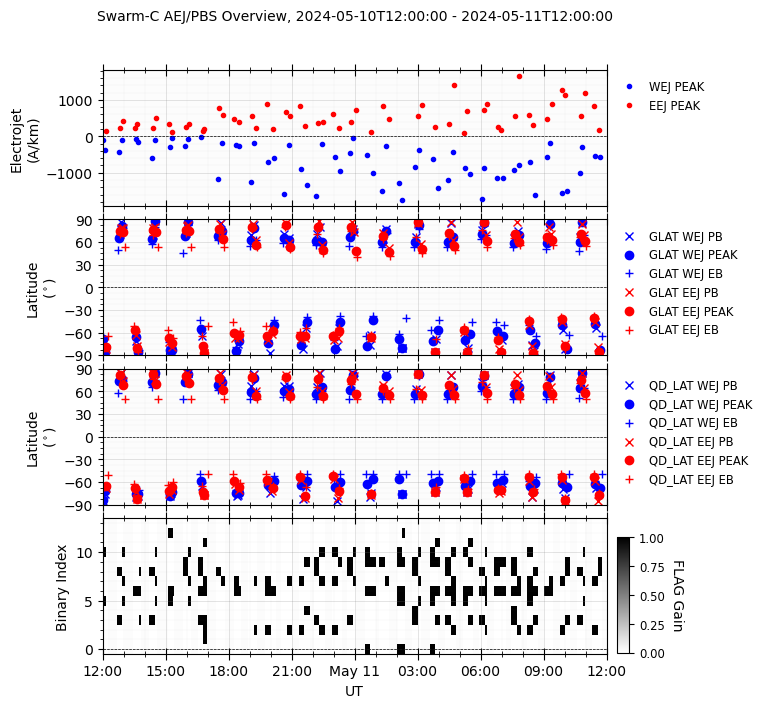
\includegraphics[width=0.7\linewidth]{files/6cd5ed9300edc4b0b9f53cad8e919269.png}

\subparagraph{Zoomed-in view with a short time span}

\begin{verbatim}
def test_swarm_AEJ_PBS_zoom():
    """Test Swarm AEJ/PBS data product
    
    """
    dt_fr = datetime.datetime(2024, 5, 10, 20, 30)
    dt_to = datetime.datetime(2024, 5, 10, 21, 0)

    db = dashboards.TSDashboard(
        dt_fr=dt_fr, dt_to=dt_to, figure_config={'figsize': (8, 8)},
        # timeline_extra_labels=['GEO_LAT', 'GEO_LON', 'APEX_LAT', 'APEX_LON', 'APEX_MLT',]  # Not applicable for very scattered data points like AEJ_PBS peaks
        )

    ds = db.dock(datasource_contents=['esa_eo', 'swarm', 'l2daily', 'aej_pbs'], sat_id='C', add_APEX=True, add_AACGM=True)

    panel_layouts = [
        [ds['WEJ_PEAK'], ds['EEJ_PEAK']],
        [
            ds['GEO_LAT_WEJ_PB'],
            ds['GEO_LAT_WEJ_PEAK'], 
            ds['GEO_LAT_WEJ_EB'],
            ds['GEO_LAT_EEJ_PB'],
            ds['GEO_LAT_EEJ_PEAK'],
            ds['GEO_LAT_EEJ_EB'],
            ],
        [
            ds['QD_LAT_WEJ_PB'],
            ds['QD_LAT_WEJ_PEAK'],
            ds['QD_LAT_WEJ_EB'],
            ds['QD_LAT_EEJ_PB'],
            ds['QD_LAT_EEJ_PEAK'],
            ds['QD_LAT_EEJ_EB'],
            ],
        [
            ds['QUALITY_FLAG_BIN_AUX'],
        ],
    ]

    db.set_layout(panel_layouts=panel_layouts)
    db.draw()
    db.add_title(title='Swarm -{} AEJ/PBS Zoom'.format(ds.sat_id), fontsize='medium', append_time=True)
    
    db.show()
test_swarm_AEJ_PBS_zoom()
\end{verbatim}

\begin{verbatim}
Create a new figure: Figure(800x800).
Searching the data product "AEJ_PBS" with the version "latest" on the server...
The file [PosixPath('/data/afys -ionosphere/data/ESA/SWARM/Level2daily/AEJ_PBS/0101/Sat_C/2024/SW_OPER_AEJCPBS_2F_20240101T000000_20241031T235959_0101.cdf')] already exists: skip downloading.
\end{verbatim}

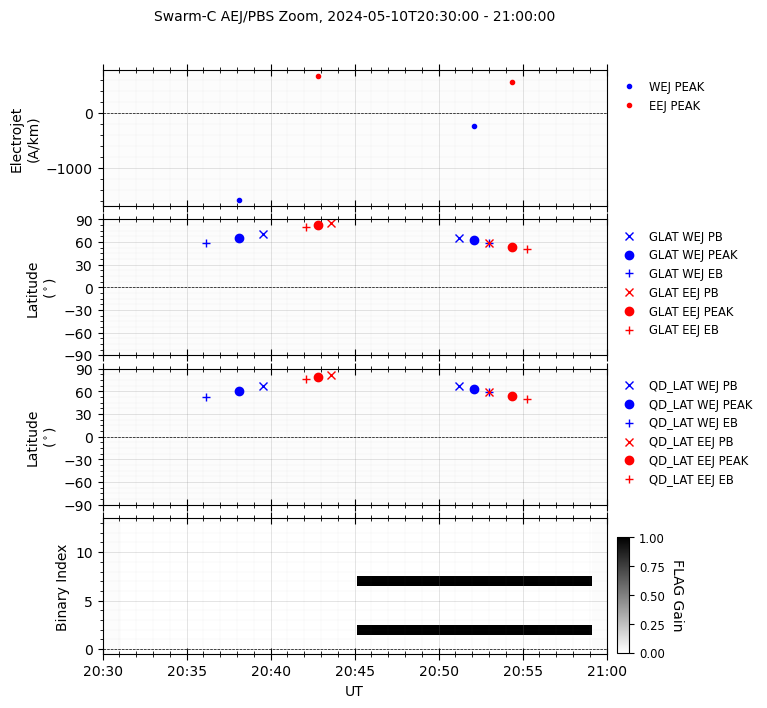
\includegraphics[width=0.7\linewidth]{files/2d6a3c8e43780af50e6393c403c30ad6.png}